%!TEX root=../Mitschrift.tex
\clearpage
\section{About Bottle}
\subsection{Was ist Bottle?}
Bottle ist ein Python web-framework welches sich besonderst durch seine performance ausgezeichnet. Hiermit können WSGI-basierte (Web Server Gateway Interface) Webanwendungen Erstellen. Es ist besonders leichtgewichtig da es sich hierbei nur um eine Datei ohne Abhängigkeiten (außer Python) handelt.\\~\\
Bottle kommt mit der Template Engine die einem erlauben Python Code in HTML Code einzubetten. (Vergleichbar mit in HTML eingebetteten JavaScript-Elementen)\\~\\
\textbf{läuft unter Python ab 2.5 und Python 3.x}
\subsection{Installation}
Da Bottle nur aus einer Datei besteht kann diese einfach von \textit{bottlepy.org} in das aktuelle Projektverzeichnis kopiert werden.
\begin{lstlisting}[language=bash]
	wget https://bottlepy.org/bottle.py
\end{lstlisting} 
Damit wird die zuletzt herausgebrachte Version kopiert. Für eine stabilere Version von Bottle wird empfohlen es mittels pip zu installieren:
\begin{lstlisting}[language=bash]
	sudo pip install bottle
\end{lstlisting} 
\subsection{Funktionalität}
\subsubsection{Herkömmliche Verwendung}
Zuerst muss bevor bottle verwendet werden kann (abgenommen es wurde installiert) importiert werden \verb|from bottle import route, run|. \\
Nun können Python-Funktionen definiert werden in denen der auszugebene Text als HTML-Code zurückgegeben wird. 
\begin{lstlisting}[language=Java]
	@route('/hello')
	def hello():
		return "Hello World!"
\end{lstlisting}
Um anzugeben wie die Funktion aufgerufen werden kann benutzen wir die Notation \verb|@route('/hello')|.\\
Als letztes müssen wir noch angeben wo die Applikation laufen soll. Das tun wir mit: \verb|run(host='localhost', port=8080, debug=True)|.\\
Nochmal die ganze Applikation:
\begin{lstlisting}
	from bottle import route, run
	
	@route('/hello')
	def hello():
		return "Hello World!"
		
		
	run(host='localhost', port=8080, debug=True)
\end{lstlisting}

Nach dem Start der Applikation kann auf diese über \verb| http://localhost:8080/hello| zugegriffen werden wobei ''/hello'' die Route auf die von uns definierte Funktion ist.

\subsubsection{Template Engine}
\section{Umsetzung}
Für den Anwendungsbeispiel wurde eine Bilddatenbank ausgewählt. Dabei hat der Nutzer die Möglichkeit Bilder hochzuladen, anzuschauen und zu löschen. Für die Datenbank wurde sqlite3 ausgewählt.

\subsection{View}
Bottle bietet die \verb|Simple Template Engine| an um die Views zu definieren. 

\subsubsection{Hauptseite - index.tpl}
Für die Hauptseite wurde eine \verb|index.tpl| erstellt, die alle hochgeladene Bilder in einer Vorschau anzeigt. Dabei wird von Python alle hochgeladen Bilder an die template engine übergeben, die dann die Inhalte rendert.

Außerdem kann auf der Hauptseite neue Bilder hochgeladen werden. Dazu wurde in HTML eine Forumlarmaske erstellt, wo die zu hochladenen Bilder ausgewählt werden können.

\begin{center}
	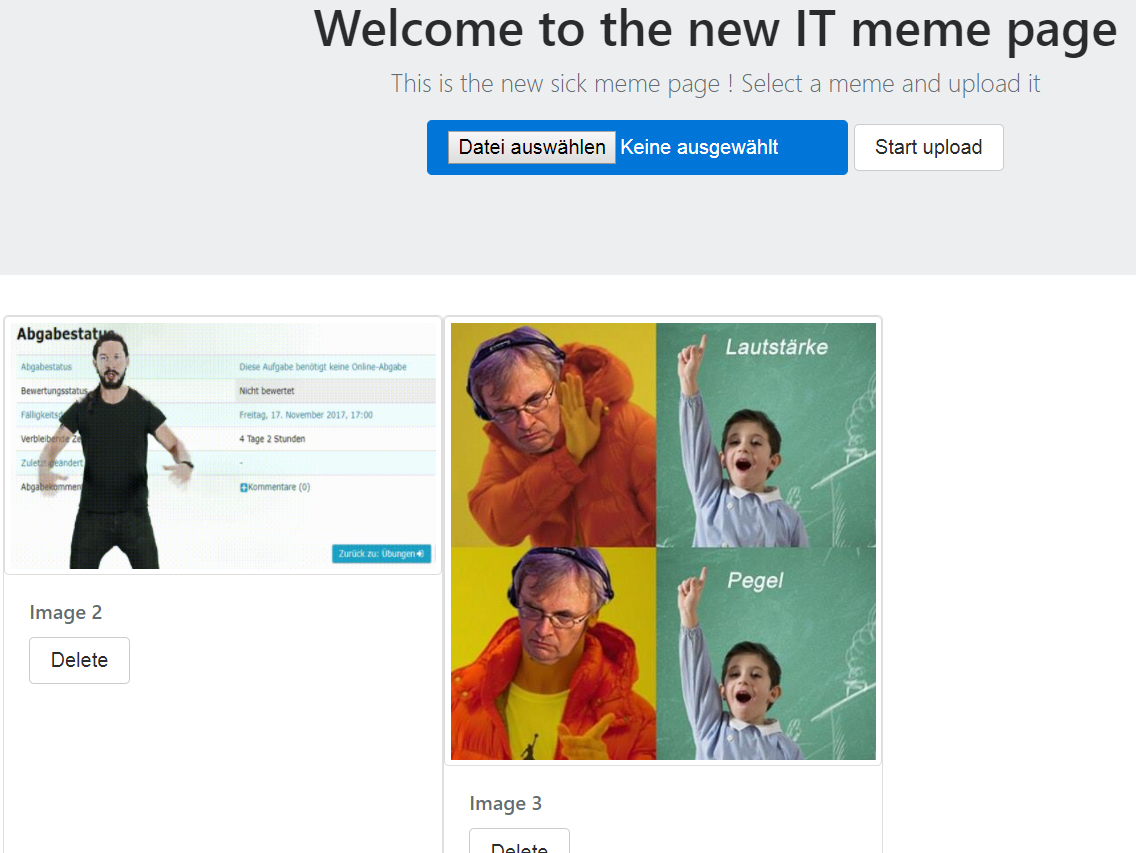
\includegraphics[width=1.0\linewidth]{images/a1.png}
\end{center}

\subsubsection{Anzeigeseite - view\_gif.tpl}
Auf dieser Seite kann das Bild im Originalformat und Originalgröße eingesehen werden. Es ist ebenfalls möglich die Bilddatei zu löschen.

% TODO: Show view page screenshot

\subsection{Die Daten}

\subsubsection{Die Bilddateien}
Die Bilddateien werden alle in einem Ordner gespeichert, da es nicht empfehlenswert ist Binärdaten direkt in einer Datenbank zu speichern. Der Pfad zu dem Bildspeicher wurde in Python definiert.

\begin{center}
	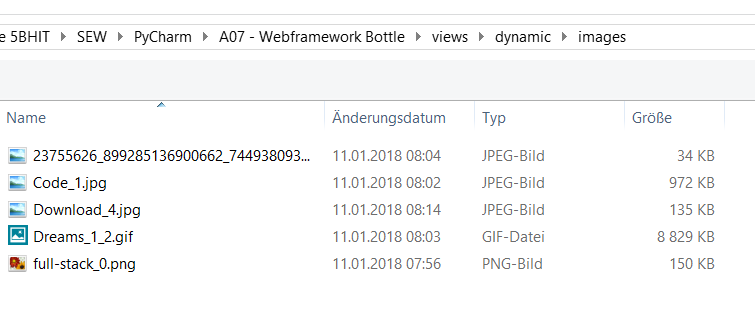
\includegraphics[width=1.0\linewidth]{images/a3.png}
\end{center}


\subsubsection{Die Datenbank}
In der Datenbank werden die Dateinamen mit einer ID referenziert. Dadurch ist es möglich schnell Bilddateien aufzufinden. 

\begin{lstlisting}[caption=Datenstruktur in SQL]
CREATE TABLE IF NOT EXISTS file_references(id INTEGER PRIMARY KEY, filename TEXT)
\end{lstlisting}

In Python wurde eine Klasse ``MemeDatabase'' erstellt, die die Schnittstelle zur sqlit3-Datenbank definiert. Es wurden Funktionen definiert die es ermöglichen:
\begin{itemize}
	\item ... Daten hinzuzufügen (save\_file\_reference)
	\item ... Daten aufzulisten (get\_all\_file\_references)
	\item ... Daten zu finden (get\_file\_reference\_or\_none)
	\item ... Daten zu löschen (remove\_file\_reference)
\end{itemize}

Durch die Datenbank ist es ebenfalls möglich weitere Spalten für später zu definieren. So könnten Spalten wie ``Titel'' oder ``Datum'' definiert werden. 

\subsection{Die ausführbare Datei main.py}
Die main.py erstellt eine neue Bottle-Instanz und definiert alle ``Routen'':
\begin{lstlisting}[caption=Applikationinstanz und Beispiel für Routen]
app = application = Bottle()
db = MemeDatabase()

<weiterer Code>

@app.route('/remove_gif/<id>')
def remove_gif(id):
	success = db.remove_file_reference(id)
	if not success:
		abort(404)
	return root()  # Show the main page
\end{lstlisting}

Damit auch alle Bildressourcen zugreifbar sind müssen auch diese routen definiert werden, da Bottle nicht automatisch die Routen zum Dateisystem definiert.
\begin{lstlisting}[caption=Routen zur Bildressourcen]
@app.route('/static/images/<picture>')
def serve_pictures(picture):
    return static_file(picture, root='views/static/images')
    
@app.route('/static/css/<css>')
def css_pictures(css):
    return static_file(css, root='views/static/css')
    
@app.route('/dynamic/images/<image>')
def serve_dyn_image(image):
    return static_file(image, root='views/dynamic/images')
\end{lstlisting}

Damit kann von jeder Seite auf die Ressource zugegriffen werden.

\subsection{Ausführung}
Für das Ausführen muss nach dem Starten von main.py die Seite \verb|localhost:8083| aufgerufen werden. Man sieht, dass die Aufrufe funktionieren, sowohl im Browser als auch in der Konsole:

\begin{center}
	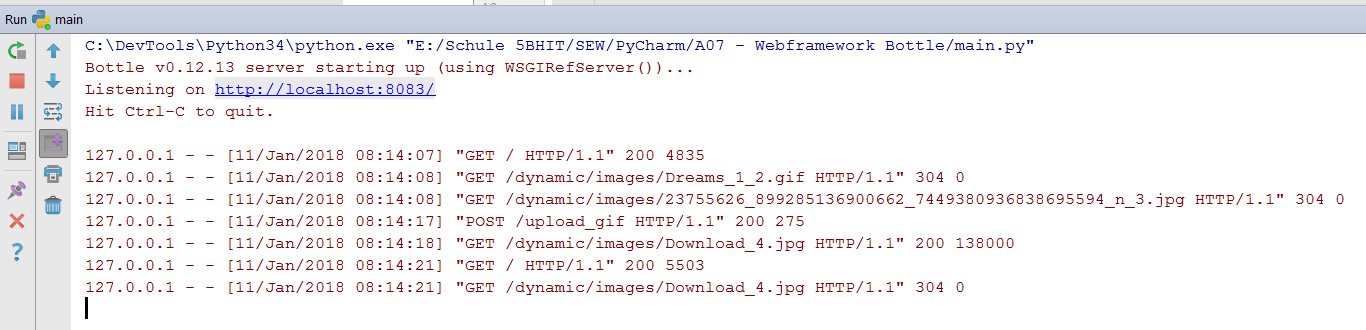
\includegraphics[width=1.0\linewidth]{images/a2.png}
\end{center}





\clearpage
\section{resources}
https://sourcemaking.com/design\_patterns
https://refactoring.guru/design-patterns/creational-patterns
https://www.philipphauer.de/study/se/design-pattern/decorator.php
